\documentclass[11pt,a4paper]{article}

\usepackage[a4paper,margin=16mm]{geometry}
\usepackage{fontspec}
\usepackage{graphicx}
\usepackage{xcolor}
\usepackage{tikz}
\usepackage{eso-pic}
\usepackage{adjustbox}
\usepackage{array}
\usepackage{tabularx}
\usepackage{paracol}
\usepackage{ragged2e}
\usepackage{microtype}
\usepackage{setspace}
\usepackage{parskip}
\usepackage{hyperref}
\usepackage{qrcode}
\usepackage{ifthen}
\usepackage{tcolorbox}
\usepackage{array}
\usepackage{multicol}
\usepackage{titlesec}
\usepackage{enumitem}
\usepackage[hidelinks]{hyperref}
\usetikzlibrary{calc,decorations.pathmorphing,decorations.markings,shapes.geometric}

\pagestyle{empty}
\setlength{\parindent}{0pt}
\hypersetup{colorlinks=true,linkcolor=peacock,urlcolor=peacock}

\definecolor{peacock}{HTML}{005F73}
\definecolor{deepPeacock}{HTML}{083C4A}
\definecolor{emerald}{HTML}{1B7F5A}
\definecolor{royal}{HTML}{1B2A6B}
\definecolor{maroon}{HTML}{7A263A}
\definecolor{gold}{HTML}{C99A2E}
\definecolor{antiqueGold}{HTML}{9E7425}
\definecolor{ivory}{HTML}{FFF8E7}
\definecolor{warmIvory}{HTML}{F8E9C8}
\definecolor{saffron}{HTML}{D87918}
\definecolor{ink}{HTML}{2B2118}
\definecolor{softBlue}{HTML}{EAF6F7}
\definecolor{nightPeacock}{HTML}{062D37}
\definecolor{royalPeacock}{HTML}{004B63}
\definecolor{lotusPink}{HTML}{B83A5A}
\definecolor{cosmicBlue}{HTML}{031820}
\definecolor{flameGold}{HTML}{F4B83F}



\IfFontExistsTF{Noto Serif Devanagari}
  {\newfontfamily\devanagarifont[Script=Devanagari,Renderer=Harfbuzz,Scale=1.08]{Noto Serif Devanagari}}
  {\IfFontExistsTF{Noto Sans Devanagari}
    {\newfontfamily\devanagarifont[Script=Devanagari,Renderer=Harfbuzz,Scale=1.08]{Noto Sans Devanagari}}
    {\IfFontExistsTF{Kohinoor Devanagari}
      {\newfontfamily\devanagarifont[Script=Devanagari,Renderer=Harfbuzz,Scale=1.08]{Kohinoor Devanagari}}
      {\newfontfamily\devanagarifont[Script=Devanagari,Renderer=Harfbuzz,Scale=1.08]{Devanagari Sangam MN}}}}

\IfFontExistsTF{Cormorant Garamond}
  {\setmainfont{Cormorant Garamond}}
  {\setmainfont{TeX Gyre Pagella}}

\IfFontExistsTF{Noto Sans}
  {\newfontfamily\sansfont{Noto Sans}}
  {\newfontfamily\sansfont{TeX Gyre Heros}}

\IfFontExistsTF{Cinzel Decorative}
  {\newfontfamily\messagefont{Cinzel Decorative}}
  {\IfFontExistsTF{Cinzel}
    {\newfontfamily\messagefont{Cinzel}}
    {\newfontfamily\messagefont{TeX Gyre Pagella}}}

\newenvironment{changemargin}[4]{%
\begin{list}{}{%
\setlength{\leftmargin}{#1}%
\setlength{\rightmargin}{#2}%
\setlength{\topmargin}{#3}%
\setlength{\bottommargin}{#4}%
}%
\item[]}
{\end{list}}

% Guest-specific values replaced by your script
\newcommand{\GuestName}{Guest Family}
\newcommand{\CheckinURL}{https://yourdomain.com/lagna/checkin.html?t=CHECKIN_TOKEN}
\newcommand{\LivestreamURL}{https://youtube.com/live/t5mw_iw27Q4}

% Set this per guest:
% \ShowVenueQRtrue  = guest is coming to venue
% \ShowVenueQRfalse = guest is not coming / livestream only
\newif\ifShowVenueQR
\ShowVenueQRtrue

\newcommand{\mr}[1]{{\devanagarifont #1}}
\newcommand{\eng}[1]{{#1}}
\newcommand{\smallcaps}[1]{{\sansfont\footnotesize\MakeUppercase{#1}}}
\newcommand{\orn}{\textcolor{gold}{\rule{12mm}{0.4pt}\hspace{2mm}$\diamond$\hspace{2mm}\rule{12mm}{0.4pt}}}
\newcommand{\revealEN}[1]{{\messagefont\fontsize{15}{19}\selectfont\textcolor{maroon}{#1}}}
\newcommand{\revealMR}[1]{{\mr{\fontsize{15}{20}\selectfont\textcolor{maroon}{#1}}}}
\newcommand{\goldline}{\begin{center}\textcolor{gold}{\rule{22mm}{0.55pt}\hspace{2mm}$\diamond$\hspace{2mm}\rule{22mm}{0.55pt}}\end{center}}
\newcommand{\storyspace}{\vspace{3.2mm}}
\newcommand{\keyword}[1]{\textcolor{maroon}{\textbf{#1}}}
\newcommand{\keyblue}[1]{\textcolor{peacock}{\textbf{#1}}}

\newcommand{\pagebg}{%
  \AddToShipoutPictureBG*{%
    \begin{tikzpicture}[remember picture,overlay]
      \fill[ivory] (current page.south west) rectangle (current page.north east);
      \shade[top color=nightPeacock,bottom color=royalPeacock] (current page.north west) rectangle ([yshift=-14mm]current page.north east);
      \shade[top color=royalPeacock,bottom color=nightPeacock] ([yshift=14mm]current page.south west) rectangle (current page.south east);
      \fill[royalPeacock] (current page.south west) rectangle ([xshift=14mm]current page.north west);
      \fill[maroon] ([xshift=-14mm]current page.south east) rectangle (current page.north east);
      \draw[gold,line width=1.45pt] ([xshift=7mm,yshift=7mm]current page.south west) rectangle ([xshift=-7mm,yshift=-7mm]current page.north east);
      \draw[gold!75!white,line width=0.45pt] ([xshift=11mm,yshift=11mm]current page.south west) rectangle ([xshift=-11mm,yshift=-11mm]current page.north east);
      \draw[peacock,line width=0.6pt] ([xshift=14mm,yshift=14mm]current page.south west) rectangle ([xshift=-14mm,yshift=-14mm]current page.north east);
      \foreach \x/\y/\r in {7/290/7,203/290/7,7/7/7,203/7/7}{
        \fill[lotusPink] (\x mm,\y mm) circle (1.4mm);
        \foreach \c/\w/\R in {100/0.9/\r,70/0.8/5.5,50/0.7/4,30/0.6/2.4}{
         \draw[gold!\c!white,line width=\w pt] (\x mm,\y mm) circle (\R mm);}
        %\draw[gold,line width=0.9pt] (\x mm,\y mm) circle (\r mm);
        %\draw[gold!30!white,line width=0.6pt] (\x mm,\y mm) circle ({\r+1}mm);
        %\draw[gold!70!white,line width=0.35pt] (\x mm,\y mm) circle (7mm);
      }
      \node[opacity=0.6] at ([xshift=28mm,yshift=-28mm]current page.north west) {\fastmandala{0.52}};
      \node[opacity=0.6,rotate=0] at ([xshift=-28mm,yshift=-28mm]current page.north east) {\fastmandala{0.52}};
      \node[opacity=0.2,rotate=0] at ([xshift=28mm,yshift=28mm]current page.south west) {\fastmandala{0.52}};
      \node[opacity=0.2,rotate=0] at ([xshift=-28mm,yshift=28mm]current page.south east) {\fastmandala{0.52}};
    \end{tikzpicture}%
  }%
}

\newcommand{\coverbg}{%
  \AddToShipoutPictureBG*{%
    \begin{tikzpicture}[remember picture,overlay]
      \fill[cosmicBlue] (current page.south west) rectangle (current page.north east);
      \node[anchor=center,inner sep=0pt,opacity=0.42] at (current page.center) {%
        \includegraphics[width=250mm,height=310mm,keepaspectratio]{assets/main-invitation.png}};
      \shade[top color=cosmicBlue!20!black,bottom color=cosmicBlue,opacity=0.86] (current page.south west) rectangle (current page.north east);
      \draw[flameGold,line width=1.7pt] ([xshift=8mm,yshift=8mm]current page.south west) rectangle ([xshift=-8mm,yshift=-8mm]current page.north east);
      \draw[gold!70!white,line width=0.45pt] ([xshift=13mm,yshift=13mm]current page.south west) rectangle ([xshift=-13mm,yshift=-13mm]current page.north east);
      %\node[opacity=0.88] at ([yshift=58mm]current page.south) {\illusionmandala{1.52}};
      %\node[opacity=0.18] at ([yshift=-28mm]current page.north) {\illusionmandala{0.95}};
    \end{tikzpicture}%
  }%
}

\newcommand{\mandala}[2]{%
  \begin{tikzpicture}[scale=#1,opacity=#2]
    \foreach \r/\c/\lw in {0.72/gold/0.45,1.15/peacock/0.48,1.68/maroon/0.42,2.25/emerald/0.45,2.85/gold/0.44,3.32/royal/0.38}{
      \draw[\c,line width=\lw pt] (0,0) circle (\r);
    }
    \foreach \a in {0,18,...,342}{
      \draw[gold,line width=0.3pt,rotate=\a] (0.45,0) .. controls (1.25,0.38) and (1.85,0.38) .. (3.1,0);
    }
    \foreach \a in {9,27,...,351}{
      \draw[peacock,line width=0.34pt,rotate=\a] (0.85,0) .. controls (1.25,0.6) and (1.95,0.6) .. (2.55,0);
    }
    \foreach \a in {0,30,...,330}{
      \draw[emerald,line width=0.16pt,rotate=\a] (0,0) -- (3.25,0);
      \fill[lotusPink,rotate=\a] (3.08,0) circle (0.045);
    }
    \node[text=gold,font=\fontsize{46}{46}\selectfont] at (0,0) {\mr{ॐ}};
  \end{tikzpicture}%
}

\newcommand{\fastmandala}[1]{%
  \begin{tikzpicture}[scale=#1]
    \draw[gold,line width=0.8pt] (0,0) circle (2.6);
    \draw[peacock,line width=1.6pt] (0,0) circle (2.05);
    \draw[maroon,line width=3.2pt] (0,0) circle (1.48);
    \foreach \a in {0,30,...,330}{
      \draw[gold,line width=0.7pt,rotate=\a] (0.35,0) .. controls (0.95,0.45) and (1.55,0.45) .. (2.45,0);
      \draw[emerald,line width=0.5pt,rotate=\a] (0,0) -- (2.6,0);
      \fill[lotusPink,rotate=\a] (2.45,0) circle (0.05);
    }
    \node[text=gold,font=\fontsize{28}{28}\selectfont] at (0,0) {\mr{ॐ}};
  \end{tikzpicture}%
}

\newcommand{\illusionmandala}[1]{%
  \begin{tikzpicture}[scale=#1]
    \foreach \r/\c/\lw in {0.75/flameGold/0.5,1.08/lotusPink/0.42,1.42/peacock/0.45,1.86/flameGold/0.48,2.32/emerald/0.42,2.82/royal/0.38,3.28/flameGold/0.5}{
      \draw[\c,line width=\lw pt] (0,0) circle (\r);
    }
    \foreach \a in {0,12,...,348}{
      \draw[flameGold,line width=0.28pt,rotate=\a] (0.28,0) .. controls (1.08,0.52) and (1.8,0.52) .. (3.12,0);
    }
    \foreach \a in {6,18,...,354}{
      \draw[lotusPink,line width=0.2pt,rotate=\a] (0.62,0) .. controls (1.18,-0.55) and (1.92,-0.55) .. (2.72,0);
    }
    \foreach \a in {0,24,...,336}{
      \draw[emerald,line width=0.2pt,rotate=\a] (0,0) -- (3.35,0);
      \fill[flameGold,rotate=\a] (3.28,0) circle (0.04);
    }
    \node[text=flameGold,font=\fontsize{44}{44}\selectfont] at (0,0) {\mr{ॐ}};
  \end{tikzpicture}%
}

\newcommand{\dharmachakra}[1]{%
  \begin{tikzpicture}[scale=#1]
    \draw[flameGold,line width=0.8pt] (0,0) circle (1.7);
    \draw[peacock,line width=0.45pt] (0,0) circle (1.22);
    \draw[flameGold,line width=0.5pt] (0,0) circle (0.26);
    \foreach \a in {0,45,...,315}{
      \draw[flameGold,line width=0.55pt,rotate=\a] (0,0.26) -- (0,1.66);
      \fill[lotusPink,rotate=\a] (0,1.72) circle (0.055);
    }
  \end{tikzpicture}%
}

\newcommand{\buddhasilhouette}[1]{%
  \begin{tikzpicture}[scale=#1]
    \fill[peacock!88!black] (0,1.85) circle (0.32);
    \fill[peacock!88!black] (-0.36,1.47) .. controls (-0.78,0.78) and (-0.68,0.1) .. (-1.32,-0.58)
      .. controls (-0.58,-0.34) and (0.58,-0.34) .. (1.32,-0.58)
      .. controls (0.68,0.1) and (0.78,0.78) .. (0.36,1.47)
      .. controls (0.18,1.28) and (-0.18,1.28) .. cycle;
    \draw[flameGold,line width=0.45pt] (0,1.85) circle (0.55);
    \draw[flameGold,line width=0.32pt] (0,0) circle (1.45);
  \end{tikzpicture}%
}

\newcommand{\watermarkmandala}[2]{%
  \begin{tikzpicture}[remember picture,overlay]
    \node at #1 {\mandala{#2}{0}};
  \end{tikzpicture}
}

\newenvironment{twocolpage}{%
  \setlength{\columnsep}{5mm}%
  \begin{paracol}{2}%
  \sloppy
}{%
  \end{paracol}
}

\newcommand{\pagetitle}[2]{%
  \begin{center}
    %\tikz[baseline=-0.6ex]\fill[gold] (0,0) -- (0.25,0.12) -- (0.5,0) -- (0.25,-0.12) -- cycle;
    \hspace{2mm}
    {\mr{\fontsize{15}{22}\selectfont\textcolor{maroon}{#1}}}\\[1mm]
    {\fontsize{15}{20}\selectfont\textcolor{peacock}{#2}}\\[-1mm]
    \orn
  \end{center}
}

\newcommand{\sectionlabel}[2]{%
  {\large\bfseries\textcolor{maroon}{#1}}\\[-1mm]
  {\large\bfseries\textcolor{peacock}{#2}}\par\vspace{2mm}
}
\newcommand{\mrsectionlabel}[2]{%
  {\mr{\large\bfseries\textcolor{maroon}{#1}}}\\[-1mm]
  {\large\bfseries\textcolor{peacock}{#2}}\par\vspace{2mm}
}


\newcommand{\profilebullet}[1]{\item {\textcolor{maroon}{\large #1}}}
\newcommand{\profilephoto}[2]{
  \includegraphics[width=\linewidth,height=#1,keepaspectratio]{#2}
}

\newtcolorbox{storybox}[2]{
  colback=#1,
  colframe=#2,
  arc=2mm,
  boxrule=0.7pt,
  left=4mm,
  right=4mm,
  top=4mm,
  bottom=4mm
}

\begin{document}



% Page Bride
\pagebg
\watermarkmandala{([yshift=-1mm]current page.north)}{0.24}
\begin{changemargin}{3mm}{3mm}{}{}

\pagetitle{\Large\textbf{दीपाली वानखेड़े}}{\Large\textbf{Deepali Wankhede}}
\vspace{4mm}
\begin{storybox}{maroon!100!white}{maroon}
  \centering
 \large\textbf{\color{antiqueGold}Gentle in expression, strong in commitment, and rooted in family values.}
\end{storybox}
\begin{minipage}[c]{0.34\linewidth}
  \begin{centering}
\profilephoto{5cm}{Deepali_intro/B_profile.jpg}\\[2mm]
\profilephoto{7cm}{Deepali_intro/B_InNature.jpg}\\[2mm]
\profilephoto{5.5cm}{Deepali_intro/B_WithOfficeFamily.jpg}\\[2mm]
\profilephoto{5cm}{Deepali_intro/B_FamilyPose1.jpg}
  \end{centering}
\end{minipage}
\hfill
\begin{minipage}[c]{0.62\linewidth}
\begin{storybox}{peacock!40!white}{peacock}
{\Large\bfseries\color{antiqueGold} Deepali}\\
{\color{peacock!100!white}\bfseries Bride}\\[1mm]
\begin{itemize}[leftmargin=5mm,itemsep=2.5mm,topsep=1mm]
\profilebullet{Comes from a close, traditional family where respect, trust, and emotional responsibility have shaped her life.}
\profilebullet{Family has always been her strongest support system; she remains deeply mindful of her parents and their values.}
\profilebullet{Completed her Master's degree and built her professional path in Information Technology.}
\profilebullet{Works in the IT sector with client communication, responsibility, and steady professional discipline.}
\profilebullet{Calm, soft-spoken, caring, and composed; she often chooses patience over reaction.}
\profilebullet{Guided by Buddhist values, family care, kindness, and thoughtfulness toward others.}
\profilebullet{Enjoys walking with her parents, talking with her mother, shopping for friends, food, and small everyday joys.}
\profilebullet{For her, marriage is a chosen bond: one person with whom she can share her whole world and explore life together.}
\end{itemize}
\end{storybox}
\vspace{2mm}
\center
\profilephoto{6.7cm}{Deepali_intro/B_sheet.png}\\
\end{minipage}

\end{changemargin}
\\

\end{center}
\end{changemargin}

\clearpage
\newpage

% Page Groom
\pagebg
\watermarkmandala{([yshift=-1mm]current page.north)}{0.24}
\begin{changemargin}{3mm}{3mm}{}{}

\pagetitle{\Large\textbf{इंदरदीप शेरे}}{\Large\textbf{Inderdip Shere}}
\vspace{4mm}
\begin{storybox}{maroon!100!white}{maroon}
  \centering
 \large\textbf{\color{antiqueGold}Curious in thought, persistent in effort, and deeply attached to family and roots.}
\end{storybox}
\begin{minipage}[c]{0.34\linewidth}
\begin{centering}
\profilephoto{5cm}{Inder_intro/G_potrait.jpeg}\\[2mm]
\profilephoto{7cm}{Inder_intro/G_InFrance.jpeg}\\[2mm]
\profilephoto{5.5cm}{Inder_intro/G_FamilyPose.JPG}\\[2mm]
\profilephoto{5cm}{Inder_intro/G_familyPose2.JPG}\\[2mm]
\end{centering}
\end{minipage}
\hfill
\begin{minipage}[c]{0.62\linewidth}
\begin{storybox}{peacock!40!white}{peacock}
{\Large\bfseries\color{antiqueGold} Inderdip}\\
{\color{peacock!100!white}\bfseries Groom}\\[1mm]
\begin{itemize}[leftmargin=5mm,itemsep=2.5mm,topsep=1mm]
\profilebullet{Family is his foundation: the place from which strength, support, and confidence radiate.}
\profilebullet{Having lived away from home since school and through his PhD, distance made his family bond even deeper.}
\profilebullet{Believes education is lifelong wealth, built through curiosity, discipline, and self-effort.}
\profilebullet{Works as a researcher in molecular simulation, in a national lab in the south of France.}
\profilebullet{Strong, stubborn, hardworking, persistent, and steady; rarely angry and famously quick to fall asleep.}
\profilebullet{Rooted in Indian culture, Hindu traditions, truthfulness to oneself, growth, and openness toward the unknown.}
\profilebullet{Enjoys running, swimming, table tennis, chess, painting, crafts, yoga, and exploring the world.}
\profilebullet{For him, marriage is a conscious equation of companionship: togetherness should increase joy and reduce life's difficulties.}
\end{itemize}
\end{storybox}
\vspace{2mm}
\center
\profilephoto{6.7cm}{Inder_intro/G_sheet.png}\\
\end{minipage}

\end{changemargin}
\\

\end{center}
\end{changemargin}
\end{document}


% Page 3
\pagebg 
\begin{changemargin}{3mm}{3mm}{1mm}{}
\watermarkmandala{([yshift=-1mm]current page.north)}{0.14}
\vspace{-4mm}
\pagetitle{कुटुंब, स्मृती आणि आशीर्वाद}{Family, Legacy, And Blessings}
%\begin{tikzpicture}[remember picture,overlay]
%  \node[opacity=0.20] at ([xshift=40mm,yshift=-144mm]current page.north west) {\dharmachakra{1.15}};
%  \node[opacity=0.18] at ([xshift=-35mm,yshift=-144mm]current page.north east) {\buddhasilhouette{0.95}};
%\end{tikzpicture}
\begin{center}
  \includegraphics[width=170mm,height=85mm,keepaspectratio]{assets/union-reception.png}
\end{center}
\goldline
\begin{twocolpage}
%\mrsectionlabel{वधू पक्ष}{Bride's Family}
\begin{centering}
{\mr{\revealMR{वधू पक्ष}}\\
\vspace{2mm}
{\mr{\textcolor{antiqueGold}{\textbf{वानखेड़े परिवार}\\
साहेबराव व मंगला वानखेड़े\\
चि. अमित यांच्यासह\\
माहेरचे परिवार:\textbf{ पोहरकर}}}}\\

\storyspace
\vspace{2mm}
\mr{\revealMR{वर पक्ष}}\\
\vspace{3mm}
\\
{\mr{\textcolor{antiqueGold}{\textbf{शेरे परिवार}\\
कै. प्रदीपकुमार व करुणा शेरे \\
चि. ट्विंकल यांच्यासह\\
माहेरचे परिवार: \textbf{जनबंधू}}}}\\
\storyspace
\vspace{3mm}
\mr{\textcolor{peacock}{या विवाहात दोन व्यक्तींचेच नव्हे, तर दोन घरांचे, चार मुळांचे, अनेक आशीर्वादांचे आणि पुढच्या पिढ्यांच्या स्वप्नांचे मंगल मिलन होत आहे.}}
}
\end{centering}

\switchcolumn
%\sectionlabel{Family Roots}{Family Roots}
\vspace{1mm}
\begin{centering}
{\revealEN{\fontsize{15}{16}\selectfont{Bride's Family }}}\\
\vspace{1mm}
{\textcolor{antiqueGold}{\textbf{Wankhede Family}\\
Sahebrao and Mangala Wankhede\\
with Amit\\
Maternal family: \textbf{ Poharkar}
}}\\

\storyspace
\vspace{2mm}
{\revealEN{\fontsize{15}{16}\selectfont{Groom's Family }}}\\
\vspace{1mm}
{\textcolor{antiqueGold}{\textbf{Shere Family}\\
Late Pradipkumar and Karuna Shere \\
with Twinkle\\
Maternal family: \textbf{ Janabhandu}
}}\\

\storyspace
\vspace{5mm}
\textcolor{peacock}{This wedding is not only the union of two people. It is the meeting of two homes, four roots, many blessings, and the dreams of generations to come.}
\end{centering}


%\vspace{2mm}
\end{twocolpage}
\begin{center}
  \includegraphics[width=0.23\linewidth,keepaspectratio]{assets/Mandala_tibet.png}\\
  \mr{\fontsize{8}{13}\selectfont\textcolor{maroon}{समेत्य च यथा भूयो व्यपयान्ति बलाहकाः ।  संयोगो विप्रयोगश्च तथा मे प्राणिनां मतः ॥}}{\small\textcolor{maroon}{\itshape{Buddhacarita 6.43}}}\\
  \mr{\fontsize{8}{13}\selectfont\textcolor{antiqueGold}{प्राणियों का एक दूसरे से संयोग जलधारा में मिलने और बिछुड़नेवाली लकड़ी या आकाश में मिलनेवाले मेघों के समान ही है।}}\\
  \small\textcolor{peacock}{The union of human beings is like the fleeting convergence of pieces of wood in a flowing stream or the brief meeting of clouds in the sky.}
\end{center}
\end{changemargin}
%\begin{center}
%  \dharmachakra{0.36}\quad
%  {\mr{\large\textcolor{maroon}{धर्मो रक्षति रक्षितः}}}\quad
%  {\itshape\textcolor{peacock}{Dharmo Rakshati Rakshitah}}\\
%  {\small Dharma protects those who protect and live by it. May this home be guided by truth, compassion, respect, and shared duty.}\\[-1mm]
%  {\small\textcolor{antiqueGold}{With the Dharma wheel's wisdom and the Buddha's compassion, may the home remain peaceful and luminous.}}
%\end{center}
\clearpage
\newpage


% Page 4
\pagebg 
\begin{changemargin}{7mm}{3mm}{1mm}{}
\watermarkmandala{([yshift=-1mm]current page.north)}{0.14}
\hspace{-7mm}
\vspace{-4mm}
\pagetitle{मंगल कार्यक्रम}{Wedding Program}
\vspace{7mm}

\begin{twocolpage}
\mrsectionlabel{पहिला दिवस : २ ऑगस्ट २०२६, रविवार }{\mr{सोहळा सुरू }}
\vspace{-1mm}
{\mr{
\textcolor{antiqueGold}{\textbf{०४:०० संध्याकाळी}} \quad \textcolor{peacock}{संगीत}\\
\textcolor{antiqueGold}{\textbf{०७:०० संध्याकाळी}} \quad \textcolor{peacock}{हळद}\\
}}

\vspace{4mm}
\mrsectionlabel{दुसरा दिवस : ३ ऑगस्ट २०२६, सोमवार}{\mr{लग्नाचा दिवस} }
{\mr{
\textcolor{antiqueGold}{\textbf{०७:०० सकाळी}} \quad  \textcolor{peacock}{हळद उतरवणे}\\
\textcolor{antiqueGold}{\textbf{१०:०० सकाळी}} \quad  \textcolor{peacock}{बौद्ध विवाह}  \\
\textcolor{antiqueGold}{\textbf{११:०० सकाळी}} \quad  \textcolor{peacock}{वैदिक विवाह} \\
\textcolor{antiqueGold}{\textbf{०२:०० दुपारी }} \quad \ \textcolor{peacock}{स्वागत समारंभ व भोजन}\\
}}

\vspace{2mm}
\mrsectionlabel{स्थळ}{\mr{आमच्यासोबत एकत्र या}}
{\mr{
\textcolor{antiqueGold}{७ वचन बँक्वेट हॉल}\\
\textcolor{peacock}{जैन मंदिराच्या बाजूला,\\
जुना भंडारा रोड, वर्धमान नगर,,\\
नागपूर, महाराष्ट्र ४४०००८, भारत}}}

\switchcolumn
\sectionlabel{\textbf{Day 1: 2 August 2026, Sunday}}{\textbf{Celebration Begins}}
\textcolor{antiqueGold}{\textbf{04:00 PM}} \quad \textcolor{peacock}{Sangeet}\\
\textcolor{antiqueGold}{\textbf{07:00 PM}} \quad \textcolor{peacock}{Haldi}\\

\vspace{4mm}
\sectionlabel{Day 2: 3 August 2026, Monday }{Wedding Day}
\textcolor{antiqueGold}{\textbf{07:00 AM}} \quad \textcolor{peacock}{Haldi Removal}\\
\textcolor{antiqueGold}{\textbf{10:00 AM}} \quad \textcolor{peacock}{Buddhist Wedding}\\
\textcolor{antiqueGold}{\textbf{11:00 AM}} \quad \textcolor{peacock}{Vedic Wedding}\\
\textcolor{antiqueGold}{\textbf{02:00 PM}} \quad \textcolor{peacock}{Reception and Lunch}\\

\vspace{4mm}
\sectionlabel{Venue}{Gather With Us}
\textcolor{antiqueGold}{7 Vachann Banquet Hall}\\
\textcolor{peacock}{Beside Jain Temple,\\
Old Bhandara Road, Wardhaman Nagar,\\
Nagpur, Maharashtra 440008, India}\\
\end{twocolpage}

\vspace{2mm}
\begin{center}
  \begin{tabular}{@{}c@{\hspace{15mm}}c@{}}
    \hspace{-7mm}\includegraphics[width=70mm,height=36mm,keepaspectratio]{assets/mehndi-haldi.png} &
    \includegraphics[width=70mm,height=36mm,keepaspectratio]{assets/haldi-preparation.png}
  \end{tabular}\\[4mm]
  %\dharmachakra{0.36}\quad{\mr{\fontsize{17}{20}\selectfont\textcolor{flameGold}{ॐ}}}\quad\dharmachakra{0.36}\\[2mm]
  {\mr{\fontsize{10}{18}\selectfont\textcolor{maroon}{आपले आशीर्वाद, स्नेह आणि उपस्थिती हाच आमचा सर्वात मोठा मंगल आशीर्वाद आहे.}}}\\
  {\messagefont\fontsize{12}{15}\selectfont\textcolor{peacock}{Your blessings, affection, and presence are our greatest gift.}}\\[3mm]
  
  
  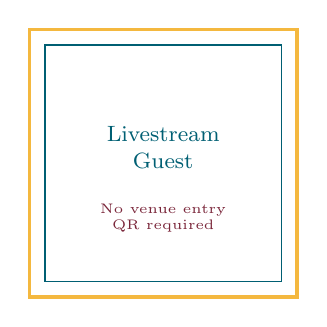
\begin{tikzpicture}
  \draw[flameGold,line width=1.2pt] (0,0) rectangle (34mm,34mm);
  \draw[peacock,line width=0.5pt] (2mm,2mm) rectangle (32mm,32mm);

  \ifShowVenueQR
    \node at (17mm,18mm) {\qrcode[height=25mm]{\CheckinURL}};
    \node[text=peacock,font=\sansfont\tiny,align=center] at (17mm,4mm)
      {\GuestName \ Family };
  \else
    \node[text=peacock,font=\sansfont\footnotesize,align=center] at (17mm,19mm)
      {Livestream\\Guest};
    \node[text=maroon,font=\sansfont\tiny,align=center] at (17mm,10mm)
      {No venue entry\\QR required};
  \fi
\end{tikzpicture}

  \vspace{2mm}
{\small\textcolor{maroon}{\mr{ थेट प्रक्षेपण / }}\textcolor{peacock}{Livestream:}}\\
{\small\url{\LivestreamURL}}
  
  %{\small\textcolor{ink}{Livestream :rtmp://a.rtmp.youtube.com/live2 }}\\
  %{\mr{\small\textcolor{ink}{थेट प्रक्षेपण : rtmp://a.rtmp.youtube.com/live2}}}\\
  
  \vspace{5mm}
  \footnotesize\textcolor{maroon}{\mr{कृपया कोणतीही भेटवस्तू किंवा आर्थिक देणगी देऊ नये. तुमची सदिच्छा आणि आशीर्वादच पुरेसे आहेत.}}\\
  \footnotesize\textcolor{antiqueGold} {We kindly request no gifts or monetary offerings. Your goodwill and blessings are enough.}
\end{center}
\end{changemargin}
\end{document}
